% This LaTeX file takes a bare input graph and applies axes, tickmarks, labels,
% etc., via TikZ and LaTeX.
%
% This approach is intended to allow user-customisable formatting of an input
% graph, beyond the limitations of the graph generating software (e.g., Maple.)

% The standalone class automatically crops the output.
\documentclass[border=0pt]{standalone}
\usepackage{tikz}   % Vector graphics support.

\begin{document}
\begin{tikzpicture}

% Standard normal cumulative distribution function graph.
\node at (0, 0) {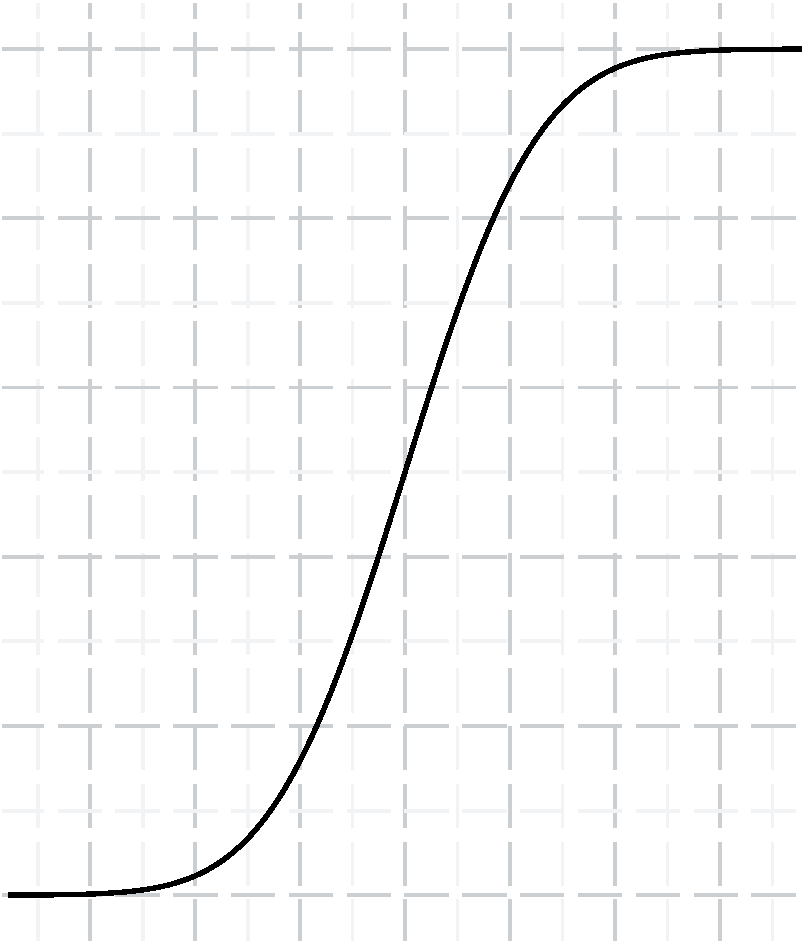
\includegraphics[width=0.3835\linewidth]{../out/graph-example-maple-bare-input.pdf}};

% Bounding rectangle.
\draw (-2.32, -2.72) rectangle (2.32, 2.72);

% Label, x-axis.
\node at (0, -3.5) {$z$};
% Label, y-axis.
\node at (-3.4, 0) {$\Phi(z)$};

% Tickmarks, major, x-axis.
\foreach \x in {-1.8020, -1.1935, ..., 2.4} \draw (\x, -2.80) -- (\x, -2.72);
% Tickmarks, minor, x-axis.
\foreach \x in {-2.1060, -1.4975, ..., 2.4} \draw (\x, -2.76) -- (\x, -2.72);
% Tickmarks, labels, x-axis.
\foreach \x [count=\xi from -3] in {-1.8020, -1.1935, ..., 2.4} \node at (\x, -3.05) {$\xi$};

% Tickmarks, major, y-axis.
\foreach \y in {-2.4521, -1.4712, ..., 2.5} \draw (-2.40, \y) -- (-2.32, \y);
% Tickmarks, minor, y-axis.
\foreach \y in {-1.9616, -0.9807, ..., 2.5} \draw (-2.36, \y) -- (-2.32, \y);
% Tickmarks, labels, y-axis.
\foreach \ytext [count=\i from 0, evaluate=\y using -2.4521 + \i*0.9808] in {$\phantom{0.}0$, $0.2$, $0.4$, $0.6$, $0.8$, $\phantom{0.}1$} \node at (-2.65, \y) {\ytext};

\end{tikzpicture}
\end{document}
